\chapter{Спектральный анализ коротких всплесков Конус-Винд} \label{sGRB_spectral_catalog}
\section{Введение}
Настоящая глава посвящена спектральному анализу 295-и коротких всплесков Конус-Винд (KW),
локализация которых была описана в Главе~\ref{IPN_catalog}. 

%В результате анализа было установлено, что для описания спектров некоторых всплесков необходима дополнительная
%степенная компонента, также обнаружено, что, вероятно, продлённое излучение значительной доли всплесков
%имеет достаточно жесткий спектр.

Глава организована следующим образом.
В разделе~\ref{sec:DATA ANALYSIS} дано описание методики спектрального анализа и
методики определения интегральных ($S$) и пиковых ($F_\rmn{peak}$) энергетических потоков.
В разделе~\ref{sec:RESULTS} приведены результаты анализа, представлены распределения параметров всплесков.
В разделе~\ref{sec:SUMMARY} полученные результаты обсуждаются в контексте физической 
классификации гамма-всплесков.

\section{Методика}\label{sec:DATA ANALYSIS}
Для каждого всплеска на основе его локализации\footnotemark вычислялась матрица отклика детектора
(см. Главу~\ref{KW_description}).
Типичный спектр короткого гамма-всплеска по данным KW состоит из подгруппы первых 
четырех спектров с временем накопления 64~мс на интервале 
от 0 до 0.256~с относительно триггера. Около 10\% всплесков имеют значимое 
излучение в пятом спектре (0.256--8.192~с). Для 4\% ярких событий
границы интервалов накопления спектров с 5-го и далее были изменены системой адаптации.

\footnotetext{Углы падения для всплесков даны в таблице~5.1 по 
ссылке \url{http://www.ioffe.ru/LEA/shortGRBs/Catalog2/Data/tables}.}

Спектр фона для коротких всплесков без продлённого излучения, как правило, 
брался на интервале $T_0+25$~с со временем накопления около 100~с, он же использовался для калибровки.
Для примерно четверти всплесков анализ многоканальных спектров был не возможен, из-за того 
что основная часть события лежала до начала измерения спектров. 
Для таких всплесков строился трехканальный спектр, с использованием отсчетов временной истории, 
накопленных за полную длительность всплеска $T_{100}$.
Из-за малого числа отсчётов (количества фотонов) для большинства всплесков 
$F_\rmn{peak}$ определялся на основе интегрального спектра. 
Только для 18 достаточно интенсивных событий можно было выделить спектр вблизи 
максимальной скорости счёта.
Итоговой набор спектров состоял из 214 интегральных многоканальных спектров 
(без учёта 18 спектров вблизи пиковой скорости счёта) и 79 трёхканальных. 
Два слабых всплеска: GRB19960325\_T69892 и GRB19980614\_T31854 имели сбои во 
временных историях и спектрах и были исключены из рассмотрения.

\subsection{Многоканальные спектры}
Спектры коротких всплесков моделировались тремя функциями: простой степенью (PL), степенью с экспоненциальным 
обрезанием (CPL) и функцией Банда (BAND), см.~Главу~\ref{KW_description}.
Процедура определения параметров моделей, описанная в Главе~\ref{KW_description}, 
для многоканальных спектров производилась в программе 
\texttt{XSPEC}\citep{Arnaud_1996ASPC} версии~12.8.0.
Для определения параметров моделей использовалась статистика $\chi^2$. 
Спектральные каналы были сгруппированы для получения не менее 10 отсчётов в канале для обеспечения 
близкой к гауссовой статистики отсчётов. Группировка по 20 и более отсчётов на канал 
приводила к исключению из анализа старших каналов спектра, 
что в некоторых случаях значительно сужало энергетический диапазон. 
В качестве нормировки модели использовался поток в диапазоне 10~кэВ--10~МэВ, 
который вычислялся с использованием модели \texttt{cflux} в \texttt{XSPEC}.
Ошибки спектральных параметров определялись для уровня 
значимости 90\%.
После определения параметров каждой из трёх спектральных моделей для спектра, 
выбиралась наиболее подходящая модель на основе различия полученного минимального $\chi^2$. 
Критерием для предпочтения модели с одним дополнительным параметром было $\Delta \chi^2 \geq 5$ 
с соответствующей вероятностью $\approx 0.025$. Было обнаружено, что такое значение предпочтительно 
для нашего набора всплесков по сравнению с часто используемым $\Delta \chi^2 \geq 6$,
так как оно даёт в два раза меньше расходящихся PL моделей, в качестве наилучших,
что критично для вычисления энергетики всплесков.


\subsection{Трёхканальные спектры}
Определение параметров PL и CPL моделей для 79 трёхканальных спектров производилось 
специально созданной программой. При этом ошибки параметров определялись методом Монте-Карло.

Для проверки методики мы сравнили результаты многоканального и трёхканального спектрального анализа
на наборе 214 всплесков с многоканальными спектрами.
Для каждого всплеска был взят  трёхканальный спектр, накопленный в течение 
интервала измерения многоканального спектра.
Затем сравнивались параметры модели, которые лучше всего описывают многоканальный спектр
с параметрами и той же модели, полученными по трёхканальному спектру.
В случае PL полученные фотонные индексы согласуются для двух типов
спектрального анализа. Для CPL модели было обнаружено, что  $\alpha$ также в целом
согласуется между двумя типами спектров. То же самое верно и для $E_\rmn{p}$, но
только в случае если значение попадает в энергетический диапазон, охватываемый трёхканальным спектром
($\lesssim 1$~МэВ), в противном случае трёхканальный анализ давал завышенное и 
плохо ограниченное значение $E_\rmn{p}$. Это показывает, что на основе данных KW 
можно получать достаточно точные значения спектральных параметров и энергетики,
даже когда многоканальные спектральные данные отсутствуют.

Поскольку аппроксимация трёхканального спектра моделью CPL имеет нулевое число степеней свободы
(и, в случае сходимости, $\chi_\rmn{CPL}^2=0$), наиболее подходящая модель 
не может быть выбрана на основе критерия $\Delta \chi^2 \geq 5$.
Поэтому, для того чтобы не переоценить энергетику всплеска, для вычисления $S$ и $F_\rmn{peak}$
использовалась модель CPL в случаях когда $E_\rmn{p}$ была ограничена снизу.

\section{Результаты}\label{sec:RESULTS}
\subsection{Спектральные параметры}
По результатам спектрального анализа было получено, что 201, 9 и 4 интегральных 
спектра наилучшим образом описываются CPL, BAND и PL, соответственно. 
Так как ни один метод основанный на использовании функции правдоподобия не даёт 
вероятности того, что конкретная модель хорошо описывает данные, в опубликованном 
каталоге были также приведены все модели параметры которых ограничены.
Для моделей CPL и BAND требовалось чтобы и $\alpha$ и $E_\rmn{p}$ имели ограниченные ошибки,
и для модели BAND дополнительно требовалось $\beta > -4$. Для исключения моделей
с большими невязками дополнительно было наложено условие на вероятность 
случайного получения заданного значения статистики $\chi^2$ 
(вероятностью нулевой гипотезы) $P> 10^{-6}$. 
Суммарно были получены параметры 473-х моделей
для интегральных спектров (210~--- CPL, 117~--- BAND и 146~--- PL).
Для всех 3-х канальных спектров кроме одного были получены параметры модели CPL, для GRB19961113\_T80522 с 
неограниченной $E_\rmn{p}$ оценки энергетики делались на основе модели PL\footnotemark. 

\footnotetext{Параметры моделей для многоканальных и трёхканальных спектров даны 
в таблице~5.2 по ссылке \url{http://www.ioffe.ru/LEA/shortGRBs/Catalog2/Data/tables}.}

На Рис.~\ref{fig:par_dist}, представлены распределения интегральных спектров по $E_\rmn{p}$ и $\alpha$.
Фотонные индексы $\alpha$ наиболее подходящих спектральных моделей распределены 
вокруг значения~$-0.5$. 
Около 66\% фотонных индексов $\alpha > -2/3$, нарушают <<линию смерти>> для 
синхротронной модели излучения~\citep{Preece_1998ApJL}, в тоже время только около 
1\% (три фотонных индекса для PL моделей) фотонных индексов $\alpha< -3/2$, 
нарушают предел охлаждения в синхротронной модели излучения \textbf{(Раскрыть смысл этих пределов)}. 
Для четырёх спектров, которые описываются степенной моделью, фотонные индексы 
находятся на мягком конце распределения $\alpha$. Для 9-и моделей BAND индексы $\beta$
распределены вблизи значения $-2.3$.
Распределение по $E_\rmn{p}$ для CPL моделей имеет максимум около 500~кэВ 
и покрывает около двух порядков величины. 
Было исследовано различие значений $E_\rmn{p}$ между моделями BAND и CPL в наборе 
моделей с ограниченными параметрами и было обнаружено, что для каждого спектра значения согласуются
в пределах ошибок на уровне 90\%.

\begin{figure}
	\begin{minipage}[h]{0.5\textwidth}
		\center{\includegraphics[width=1\textwidth]{gDistAlpha_ru.eps} \\ а)}
    \end{minipage}
    \hfill
    \begin{minipage}[h]{0.5\textwidth}
		\center{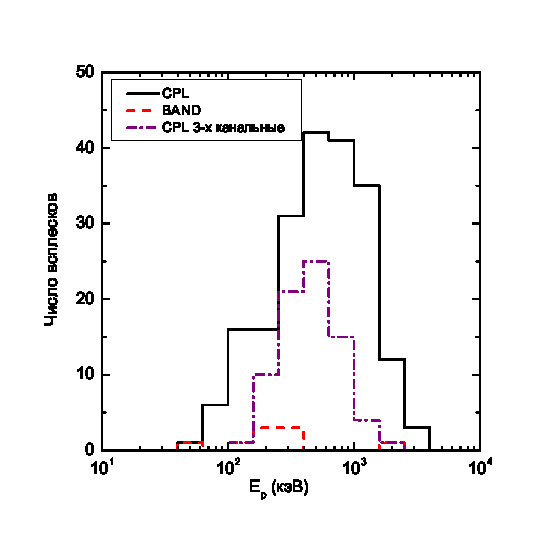
\includegraphics[width=1\textwidth]{gDistEp_ru.eps} \\ б)}
	\end{minipage}
    \caption{
    Распределение $\alpha$~(а) и $E_\rmn{p}$~(б), полученных 
    в результате моделирования интегральных спектров. Распределение для каждой модели
    показано отдельно.
    \label{fig:par_dist} }
\end{figure}

\subsection{Всплески с дополнительной спектральной компонентой}
Для трёх ярких всплесков была получена низкая достоверность моделирования 
интегральных спектров ($P<0.001$) для всех трёх использованных моделей. 
Детальное рассмотрение этих всплесков выявило причину малых значений $P$.
Всплеск GRB20060306\_T55358, с $P \approx 10^{-4}$, имеет сильную 
спектральную эволюцию~--- жесткость спектра уменьшается в течении всплеска, 
что приводит к систематическому расхождению с модельными спектрами (BAND и CPL).
Однако, модель BAND хорошо описывает ($P>0.05$) отдельные спектры этого яркого всплеска.
Было обнаружено, что интегральные спектры двух других всплесков GRB19960908\_T25028 и GRB20031214\_T36655
хорошо описываются суммой функций CPL и PL.
Помимо перечисленных всплесков, явные систематические отклонения модели от спектра
были обнаружены для интегрального спектра GRB19980205\_T19785 ($P=0.08$), 
который также хорошо аппроксимируется суммой CPL+PL.
 
Параметры CPL+PL аппроксимаций интегральных спектров описанных всплесков приведены в Таблице~\ref{tab:extra_comp}. 
Степенная компонента этих спектров, которая также детектируется в большинстве отдельных спектров,
является достаточно жесткой ($\alpha \sim -2$) и даёт основной вклад в спектр на  
энергиях ниже $\sim 50$--100~кэВ, и должна доминировать на энергиях $\gtrsim 10$~МэВ.
Жесткая CPL компонента имеет $E_\rmn{p}\sim(1.5\textrm{--}2)$~МэВ и достаточно пологий
фотонный индекс $\alpha > -1$).
Все перечисленные всплески находятся среди 10\% наиболее интенсивных всплесков
в смысле интегральных энергетических потоков, при этом
GRB20031214\_T36655 и GRB20060306\_T55358 имеют наибольшие потоки в наборе.

{\renewcommand\tabcolsep{3pt}
\begin{table} [h]
 \centering
  \caption{Параметры интегральных спектров с дополнительной компонентой (CPL+PL).}
  \label{tab:extra_comp}
  \scriptsize
  \begin{center}
  \begin{tabular}{ccccccccc}
  \hline
  \hline
  Обозначение & $\alpha_\rmn{CPL}$ & $E_\rmn{p,CPL}$, & Flux$_\rmn{CPL}$,$10^{-6}$ & $\alpha_\rmn{PL}$ & 
      Flux$_\rmn{PL}$, $10^{-6}$ & $\chi^2/\rmn{dof}$ \\
  всплеска &   & МэВ & эрг~см$^{-2}$~с$^{-1}$ &  & эрг~см$^{-2}$~с$^{-1}$ & (вер.) \\
  \hline  
GRB19960908\_T25028 & $-0.5(-0.5,+0.8)$ & $1.53(-0.28,+0.36)$ & $27.3(-8.0,+7.0)$   & $-2.1(-0.4,+0.2)$ & $8.7(-5.2,+8.8)$  & 77/63 (0.11) \\
GRB19980205\_T19785 & $-0.7(-0.6,+1.2)$ & $1.81(-0.67,+1.33)$ & $13.2(-5.6,+6.2)$   & $-2.2(-0.5,+0.2)$ & $5.4(-3.0,+3.9)$  & 40/55 (0.94) \\
GRB20031214\_T36655 & $-0.3(-0.1,+0.1)$ & $1.91(-0.08,+0.08)$ & $274.6(-13.4,+12.4)$& $-2.0(-0.4,+0.2)$ & $10.6(-5.6,+8.6)$ & 87/75 (0.15) \\
\hline
\end{tabular}
\end{center}
\end{table}
}

\subsection{Интегральные и пиковые потоки}
Значения $S$ и $F_\rmn{peak}$ вычислялись с использованием энергетического потока,
полученного для наиболее подходящей спектральной модели в диапазоне 10~кэВ--10~МэВ.
Так как интервал накопления спектра обычно отличался от $T_{100}$, применялась 
коррекция, которая учитывала излучение лежащие вне интервала накопления спектра 
для вычисления $S$.
Для коротких всплесков с продлённым излучением интегральные энергетические потоки 
вычислялись отдельно для EE и начального импульса (см. Раздел~\ref{sec:EE}).
Значение $F_\rmn{peak}$ вычислялось на масштабе 16~мс с использованием наиболее 
подходящей спектральной модели для спектра вблизи максимальной скорости счёта.
Для получения $F_\rmn{peak}$ поток по модели умножался на отношение 
пиковой скорости счёта на масштабе 16~мс к средней скорости счёта за интервал 
накопления спектра. Обычно для коррекции использовались отсчёты в группах каналов
G2+G3, G1+G2 только G2 или G1+G2+G3 в зависимости от жесткости спектра.
Значения $S$ и $F_\rmn{peak}$ были получены для 293-х всплесков.
Распределения всплесков по $S$ и $F_\rmn{peak}$ показаны на рисунке~\ref{fig:fl_pf_dist}.

Следует отметить, что для нескольких очень интенсивных и сильно переменных всплесков 
(GRB19970704\_T04097, GRB20031214\_T36655, GRB20051103\_T33943, GRB20060306\_T55358,
GRB20070201\_T55390 и GRB20070222\_T27115)
значения $F_\rmn{peak}$ (и в меньшей степени $S$) могут быть недооценены на основе описанного анализа
в $\sim1.5$--2 раз, из-за того что мёртвое время в спектрах оценивалось на основе предположения о 
постоянстве скорости счёта в интервале накопления.

\begin{figure}
    \begin{minipage}[h]{0.5\textwidth}
		\center{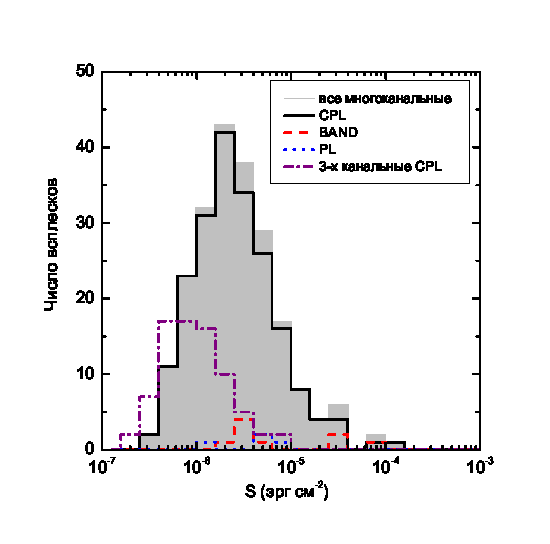
\includegraphics[width=1\textwidth]{gDistS_ru.eps} \\ а)}
    \end{minipage}
    \hfill
    \begin{minipage}[h]{0.5\textwidth}
		\center{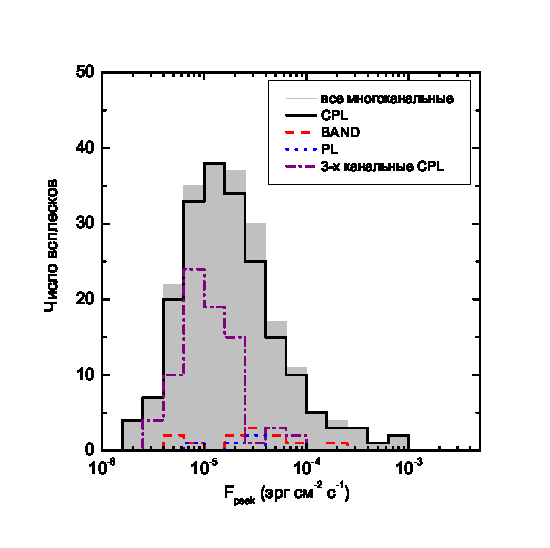
\includegraphics[width=1\textwidth]{gDistPF_ru.eps} \\ б)}
	\end{minipage}
\caption{
    Распределение интегральных~(а) и пиковых энергетических потоков~(б)
    Серым на каждой панели показано суммарное по всем моделям распределение для 214
    многоканальных спектров, распределения для каждой модели показаны отдельно. 
    Штрихпунктирной линией показаны распределения для 79 трёхканальных спектров.
    \label{fig:fl_pf_dist} }
\end{figure}

\subsection{Короткие всплески с продлённым излучением}\label{sec:EE}
Продлённое излучение (EE), которое следует после короткого начального импульса (IP),
наблюдалось у некоторой части коротких всплесков, зарегистрированных различными экспериментами:
\textit{CGRO}-BATSE~\citep{Burenin_2000AstL, Norris_and_Bonnel_2006ApJ, Bostanci_2013MNRAS}, 
KW~\citep{Mazets_2002astroph, Frederiks_2004ASPC}, 
\textit{INTEGRAL}-SPI-ACS~\citep{Minaev_2010AstL}, 
\textit{Swift}-BAT~\citep{Norris_2011ApJ, Sakamoto_2011ApJS}, 
и \textit{Fermi}-GBM~\citep{Kaneko_2015MNRAS}. 
Поиск кандидатов в короткие всплески с EE был произведён в Главе~\ref{KW_GRB_classification}, 
было обнаружено 31 событие. Хотя яркий начальный импульс GRB~070207~\citep{Golenetskii_2007GCN6089}
удовлетворяет критериям короткого всплеска ($T_{50}=0.010\pm0.004$~с) с $E_\rmn{p}\sim 300$~кэВ,
очень яркое и жесткое ($E_\rmn{p}\sim 1.5$~МэВ последующие излучение, которое лишь формально может
считаться EE, предполагает, что это событие~--- длинный/жесткий всплеск с коротким прекурсором,
схожий по морфологии с двумя другими всплесками KW, GRB~000115 
и GRB~001020~\citep{Hurley_2000GCN859}

%We defined the following search criteria: 
%the burst initial pulse should meet our criteria for a short GRB, i.e. have $T_{50}<0.6$~s;
%and the remaining part of burst (EE) shouldn't exhibit peaks with prominent spectral evolution. 
%Applying these criteria to the full KW sample, we found 31 short GRBs with EE candidates. 
%Only for 22 events EE was bright enough to allow spectral analysis.
%The initial pulses of these events are classified in Table~\ref{tab:durations} as Iee or Iee/II.

Только для 21-го события, из оставшихся 30-и, интенсивность EE была достаточной для спектрального анализа.
Для 15-и всплесков наилучшей спектральной моделью для EE является PL и для 6~--- CPL.   
Фотонные индексы модели PL находятся в диапазоне от $-2.6$ до $-1.4$ с медианой $-1.6$,
и в диапазоне от $-1.4$ до $-0.3$ с медианой $-1.2$ для модели CPL.
Значения $E_\rmn{p}$ находятся в диапазоне от $\approx160$~кэВ до $\approx 2.2$~МэВ с медианой $\approx300$~кэВ
и средним геометрическим $\approx370$~кэВ. 
Для указанного 22-го всплеска было вычислено отношение потоков EE/IP, 
которое изменяется в пределах от 0.06 до 15 с медианой 3.3. 
Из шести всплесков, у которых EE описывается моделью CPL, у четырёх $E_\rmn{p}$ EE 
меньше чем у начального импульса и для двух всплесков, GRB19950526\_T16613 и GRB20090720\_T61379, 
наблюдается обратная ситуация, причем второй всплеск имеет экстремально
жесткое EE ($E_\rmn{p} = 2.2(-1.0,+2.4)$~МэВ).


\section{Обсуждение результатов}\label{sec:SUMMARY}
В главе представлены результаты спектрального анализа 293-х коротких гамма-всплесков,
зарегистрированных в эксперименте Конус-Винд, этот набор составляет $\sim 15$\% 
от полного числа всплесков, зарегистрированных за первые 15 лет работы инструмента.
Набор включает $\sim 70$\% всплесков Типа~I, $\sim 8$\% Типа~II и $\sim 12$\%
имеют неопределённый тип (I или~II). Доля коротких всплесков с продлённым 
излучением составляет $\sim 10$\%.

Суммарно было проанализировано 253 многоканальных спектров: 214 интегральных,
18 пиковых и 21 спектр продлённого излучения; и 79 трёхканальных спектров.
Таблица~\ref{tab:pardist} содержит медианы и 90\% интервалы распределений спектральных
параметров и энергетики, полученных в главе. В первой колонке дано название параметра;
во второй тип спектральных данных: многоканальный <<mult>> или трёхканальный <<3ch>> спектр;
последующие колонки содержат медианы и 90\% интервалы для распределений
$\alpha$, $E_\rmn{p}$, $S$ и $F_\rmn{peak}$. Для распределения по $\beta$
медиана и 90\% интервал составляют $-2.28$ и $[-3.15,-1.74]$, соответственно.

Наибольшие $E_\rmn{p}$ измеренные для коротких всплесков KW составляют $\sim 3$~МэВ: 
$E_\rmn{p} = 3.55(-0.71,+0.85)$~МэВ было получено для GRB20090510\_T01381
(GRB 090510~\citep{Ackermann_2010ApJ_716_1178A});
более мягкие всплески GRB19970704\_T04097 и GRB20080611\_T04742 имеют $E_\rmn{p} \approx 3.3$~МэВ.
Практически все всплески с $E_\rmn{p} \lesssim 200$~кэВ классифицированы как Тип~II или Тип~I/II
и, вероятно, представляют собой популяцию отличную от более жестких всплесков (см. обсуждение ниже).

\begin{deluxetable}{ccccccc}
\tabletypesize{\scriptsize}
\tablecaption{Median Values and 90\% CI for the best-fit model parameter distributions\label{tab:pardist}}
\tablewidth{0pt}
\tablehead{
\colhead{Model} &
\colhead{Data Type\tablenotemark{a}} &
\colhead{$\alpha$} &
\colhead{$\beta$} &
\colhead{$E_\rmn{p}$} &
\colhead{Fluence} &
\colhead{Peak Flux} \\
\colhead{} &
\colhead{} & 
\colhead{} &
\colhead{} &
\colhead{(keV)} &
\colhead{($10^{-6}$~erg~cm$^{-2}$)} &
\colhead{($10^{-5}$~erg~cm$^{-2}$~s$^{-1}$)} \\
}
\startdata   
   PL  & mult & $-1.78(-0.21,+0.17)$ &    \nodata          &     \nodata       & $ 4.1(-2.7,+1.6)  $ & $ 2.1(-1.3,+0.9)  $ \\
  CPL  &      & $-0.49(-0.68,+0.91)$ &    \nodata          & $554(-439,+1253)$ & $ 2.3(-1.8,+11.6) $ & $ 1.5(-1.2,+11.3) $ \\
 BAND  &      & $0.28(-1.10,+1.07) $ & $-2.28(-0.69,+0.45)$ & $244(-195,+105)$  & $ 3.8(-1.9,+35.3) $ & $ 2.8(-2.4,+4.5)  $ \\
  all  &      &   \nodata            &     \nodata         &    \nodata        & $ 2.4(-1.9,+17.7) $ & $ 1.6(-1.2,+11.2) $ \\
  CPL  & 3ch  & $-0.36(-0.88,+1.26)$ &     \nodata         & $459(-269,+721)$  & $ 0.9(-0.6,+2.5)  $ & $ 1.0(-0.6,+3.0)  $ \\
\enddata
\tablenotetext{a}{Multichannel spectrum~--- ``mult'' or tree chamnnel spectrum~--- ``3ch''}
\end{deluxetable}

Результаты анализа подтверждают, что спектры большей части коротких всплесков хорошо
описываются моделью CPL с жестким $\alpha \sim -0.5$ и $E_\rmn{p}$ в диапазоне 100~кэВ--2~МэВ.
В представленном анализе только $\sim 4$\% коротких всплесков KW описываются моделью BAND.
Среди 5\%  всплесков с наибольшим $S$, 20\% описываются моделью BAND; для описания 
оставшихся 80\% требуется $\beta \lesssim -2.5$, в большинстве случаев неограниченное снизу.
Это предполагает, что отсутствие степенного поведения спектра на больших энергиях,
обнаруженное для большей части ярких коротких всплесков, по видимому является внутренним
свойством всплесков, а не связанно с низкой статистикой отсчётов на больших энергиях.

В данном разделе не ставилась задача проверки применимости более сложных моделей
для описания спектров коротких всплесков.
Однако, среди 214-и всплесков с многоканальными спектрами было обнаружено три
события, для описания которых необходима дополнительная жесткая степенная 
спектральная компонента с фотонным индексом $\sim -2$. Эти всплески входят в 10\%
наиболее интенсивных событий из набора. Отношение энергетических потоков PL
компоненты к CPL находится в диапазоне от 0.03 для GRB20031214\_T366655 до
0.4 для GRB19980205\_T19785. Обнаруженная компонента может иметь ту же природу,
что и обнаруженная в GRB~081024B~\citep{Abdo_2010ApJ_712_558A} и 
GRB~090510~\citep{Ackermann_2010ApJ_716_1178A} на основе данных \textit{Fermi}-GBM и~LAT.
GRB~081024B не был зарегистрирован KW триггерном режиме, GRB~090510 (GRB20090510\_T01381)
содержится в нашем наборе. Для описания спектра последнего всплеска степенная 
компонента не требуется, верхний предел на поток степенной компоненты с фотонным 
индексом $-1.7$ составляет $\sim 1 \times 10^{-6}$~эрг~см$^{-2}$~с$^{-1}$ для 
уровня значимости 90\%. Соответствующий предел на отношение потока PL компоненты 
к потоку в основной компоненте составляет $\lesssim 0.02$ на уровне значимости 90\%.
\textbf{Написать подробней про эти всплески, добавить картинки.}

\subsection{Сравнение коротких всплесков KW с BATSE и GBM}
Результаты представленного спектрального анализа были сопоставлены с данными
других экспериментов.
Наибольшие наборы данных по GRB в широком спектральном диапазоне получены экспериментами
\textit{CGRO}-BATSE\footnote{\url{http://heasarc.gsfc.nasa.gov/W3Browse/cgro/bat5bgrbsp.html}}
(в диапазоне 20~кэВ--2~МэВ~\citep{Goldstein_2013ApJS}) и 
\textit{Fermi}-GBM\footnote{\url{http://heasarc.gsfc.nasa.gov/W3Browse/fermi/fermigbrst.html}}
(в диапазоне 8~кэВ--40~МэВ~\citep{Gruber_2014ApJS}). 
Настоящий анализ содержит примерно в два раза коротких всплесков, чем каталог GBM, 
в более узком диапазоне энергий, и в $\sim 1.5 $ раза меньше чем набор BATSE, 
но в более широком диапазоне энергий.

Из каталога BATSE~5B было выбрано 427 всплесков с $T_{90}<2$~с и с интервалом 
накопления интегрального спектра короче 10~с. На основе критерия $\Delta \chi^2>6$
всплески имеют следующую статистику наиболее подходящих моделей:
11~--- BAND, 225~--- CPL и 191~--- PL.
Из второго каталога GBM было выбрано 146 всплесков с $T_{90}<2$~с. Наиболее подходящие модели,
по данным каталога распределены так: 3~--- BAND, 67~--- CPL и 76~--- PL;
всплески описываемые степенной моделью с изломом (около пяти событий) были 
исключены из сравнения.

Отношение числа всплесков, описываемых BAND и CPL моделями, мало ($\lesssim 5$\%)
для всех наборов. Было проверено согласуются ли распределения по $\alpha$ и 
$E_\rmn{p}$ модели CPL между инструментами. Двусторонние p-значение 
теста Колмогорова-Смирнова для двух наборов ($P_\rmn{KS}$) для распределений 
KW и GBM по $\alpha$ и $E_\rmn{p}$ равны 10\% и 25\%, соответственно, в то время 
как для сравнений KW и BATSE, и GBM и BATSE $P_\rmn{KS}<1$\%.
Набор BATSE имеет медиану $\alpha=-0.33$ в то время как медианы KW и GBM равны
$\alpha=-0.49$ и $\alpha=-0.50$, соответственно.
Медианы распределений по $E_\rmn{p}$ равны $\approx 400$~кэВ для BATSE и 
$\approx 550$~кэВ для KW и GBM.
Таким образом результаты KW хорошо согласуются с данными GBM и хуже с данными BATSE.

Доля всплесков, наилучшим образом описываемых моделью PL, сильно отличаются у KW и
других инструментов:
2\% (5\% используя критерий $\Delta \chi^2 > 6$)~--- KW, 52\%~--- GBM и 55\%~--- BATSE.
Причина достаточно большой доли PL моделей у BATSE и GBM была детально проанализирована.
Для более устойчивого сравнения были выбраны всплески с $S>5.5\times 10^{-7}$~эрг~см$^{-2}$,
данный порог примерно соответствует наименьшему $S$, полученному для всплесков KW с многоканальными
спектрами. Полученные поднаборы 138 (BATSE) и 49 (GBM) GRBs содержали 29 (21\%) и 3 (6\%) моделей PL, соответственно. 
Таким образом, в схожем диапазоне интегральных энергетических потоков доли PL моделей
согласуются для KW и GBM.
Среди моделей CPL с ограниченными параметрами для указанных 29 всплесков BATSE,
17 имеют $1\sigma$ верхний предел $E_\rmn{p}$, превышающий верхнюю границу 
спектрального диапазона  BATSE (2~МэВ). Оставшиеся 12 всплесков составляют 9\% от поднабора. 
Следовательно, можно считать, что основным источником избытка PL моделей для коротких 
всплесков BATSE и GBM является большое количество слабых всплесков (с низким $S$),
для которых более сложная модель не может быть предпочтительна из-за низкой статистики отсчётов.
Для всплесков BATSE дополнительным фактором, влияющим на увеличение доли PL моделей, 
является относительно узкий спектральный диапазон.

\subsection{Короткие всплески с EE}
Было обнаружено, что 30 всплесков из набора 1939 KW гамма-всплесков зарегистрированных
с 1994 по 2010 гг. могут быть классифицированы как короткие всплесков с EE, 
основываясь на длительности начального импульса и отсутствие в последующем излучении 
заметной спектральной эволюции. Из них, 21 всплеск имел интенсивность EE достаточную
для анализа многоканальных спектров. Для шести из этих всплесков спектр EE описывается
моделью с изломом (CPL) с достаточно высокой $E_\rmn{p} \sim 160$~кэВ--2.2~МэВ.
Начальные импульсы двух из них были классифицированы как типы Iee/II и они вероятно
являются длинными всплесками с короткими начальными импульсами. Оставшиеся четыре всплеска 
являются <<стандартными>> короткими всплесками с продлённым излучением на основании 
формы временного профиля. Подобные спектры был обнаружены у двух из 19 всплесков BATSE~\citep{Bostanci_2013MNRAS}
и у четырёх из 14 всплесков GBM~\citep{Kaneko_2015MNRAS}. 
Полученные соискателем результаты дают дополнительное свидетельство в пользу наличия 
достаточно жесткого продлённого излучения у коротких гамма-всплесков. 

Набор коротких всплесков с продлённым излучением KW включает два всплеска, 
где EE наблюдалось на BATSE, и три, где EE наблюдалось GBM. 
Результаты спектрального анализа этих всплесков (включая GRB20090831\_T27393 с жетким EE, 
$E_\rmn{p} \approx 215$~кэВ) по данным KW согласуются с результатами упомянутых инструментов.
Всплеск GRB20090720\_T61379 с экстремально жестким EE ($E_\rmn{p} \approx 2.2$~МэВ) 
был зарегистрирован GBM. Хотя всплеск не был включён в набор~\citep{Kaneko_2015MNRAS},
параметры интегрального спектра этого всплеска по данным KW согласуются с полученными 
по данным GBM.
 
Яркий близкий всплеск GRB~060614, который был классифицирован как короткий 
всплеск с EE~\citep{Gehrels_2006Nature} был зарегистрирован KW ($T_0$(KW)=45831.590~с;~\citep{Golenetskii_GCN5264}).
Этот всплеск не был включён в наш набор коротких всплесков из-за большой 
длительности начального импульса $T_{50}=2.7 \pm 0.3$~с.

\subsection{Кандидаты в гигантские вспышки SGR}
Яркий начальный импульс гигантской вспышки (GF) источника мягких повторяющихся гамма-всплесков, 
произошедшей в близкой галактике, может выглядеть в данных гамма детектора как короткий гамма-всплеск. 
Верхней предел на частоту GF на основе локализаций коротких свсплесков KW был
получен в Главе~\ref{SGR_GF_search}. При этом было обнаружено только два кандидата:
GRB~051103 (GRB20051103\_T33943) в группе галактик M81/M82~\citep{Frederiks_2007AstLett} и 
GRB~070201 (GRB20070201\_T55390) в галактике M31~\citep{Mazets_2008ApJ}.
Оба события находятся среди 10\% наиболее интенсивных событий на основе интегрального 
энергетического потока. Спектральные параметры всплесков являются типичными для 
набора коротких всплесков KW.
Избыток отсчётов, наблюдаемый вплоть до 90~с после триггера GRB~070201, 
был интерпретирован как хвост гигантской вспышки~\citep{Mazets_2008ApJ}.
Значимость избытка составляет $4.3\sigma$, поэтому он не был обнаружен при 
поиске продлённого излучения (с порогом $5\sigma$).

\subsection{Неоднородность набора коротких всплесков}
На рис.~\ref{fig:EpT50} показано соотношение $E_\rmn{p}$, для наиболее подходящей CPL модели,
и длительности всплеска $T_{50}$. Всплески Типа~I, в среднем, короче и жестче 
($E_\rmn{p}\gtrsim 200$~кэВ), чем всплески Типа~II, что подтверждает классификацию,
полученную на основе распределения жесткость-длительность.
Среди 4-х всплесков наилучшим образом описываемых моделью PL, два всплеска принадлежат к типам I и II,
и два имеют неопределённый тип (I/II). Явный недостаток всплесков с $E_\rmn{p}\lesssim 100$~кэВ,
скорее всего связан с эффектом селекции. 
Распределение по длительности начальных импульсов коротких всплесков типа~I с EE (Iee) согласуется с 
распределением для обычных коротких всплесков типа~I, о чем свидетельствует p-значение
теста Колмогорова-Смирнова $P_\rmn{KS}=0.5$. Также было обнаружено, что
начальные импульсы всплесков типа Iee, в среднем, жестче ($E_\rmn{p}$ в $\sim 1.5$ раза выше),
чем всплески типа~I ($P_\rmn{KS} = 0.01$). В заключении были сопоставлены распределения 
всплесков типов Iee и~I по $S$ и $F_\rmn{peak}$, для пар распределений 
была получена $P_\rmn{KS} \sim 0.01$, что свидетельствует о различие распределений,
при этом начальные импульсы всплесков с EE, в среднем, более интенсивные.

\begin{figure}
    \begin{minipage}[h]{0.5\textwidth}
		\center{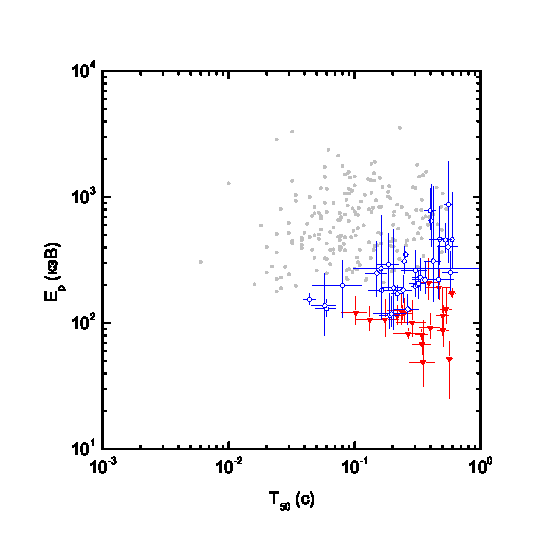
\includegraphics[width=1\textwidth]{gEpvsT50TypesII_ru.eps} \\ а)}
    \end{minipage}
    \hfill
    \begin{minipage}[h]{0.5\textwidth}
		\center{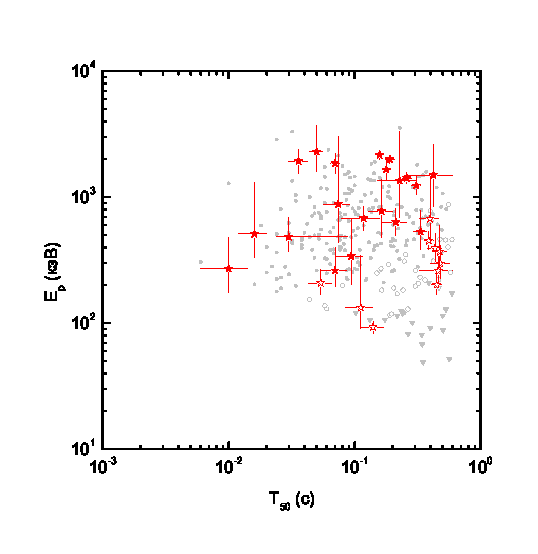
\includegraphics[width=1\textwidth]{gEpvsT50ipEE_ru.eps} \\ б)}
	\end{minipage}

\caption{
    Соотношение $E_\rmn{p}$ и $T_{50}$ (только для модели CPL).
    На панели~(а) показаны всплески типа~I (серые точки), типа~II (красные треугольники)
    и всплески неопределённого типа, I или~II (синие окружности).
    На панели~(б) показаны всплески типа~I с EE (заполненные красные звёзды)
    и всплески неопределённого типа Iee/II (пустые красные звёзды)
    Для всплесков типа~I ошибки не показаны. 
    \label{fig:EpT50}}
\end{figure}

На рис.~\ref{fig:EpvsFPandFL} приведены соотношения $E_\rmn{p}$ с $S$ и $F_\rmn{peak}$.
Распределение 79 слабых всплесков с трёх-канальными спектрами по спектральным параметрам 
и $F_\rmn{peak}$ схоже с более интенсивными событиями, эти всплески являются продолжением
распределения коротких/жестких (Тип~I) всплесков в область низких $S$  на диаграмме $E_\rmn{p}$--$S$.
Явным выбросом из  $E_\rmn{p}$--$F_\rmn{peak}$ распределения является предполагаемая 
GF в галактике M31, что подкрепляет свидетельства в пользу отличной от GRB природы этого события.
Всплески типов I и~II занимают практически не пересекающиеся области на диаграмме $E_\rmn{p}$--$S$.
Всплески типа~I образуют вытянутое распределение, которое, в среднем, подчиняется 
соотношению $E_\rmn{p} \propto S^{1/2}$. Всплески типа II образуют небольшую группу событий
с низкой $E_\rmn{p}$, которая представляет собой малую часть распределения длинных всплесков.
На плоскости $E_\rmn{p}$--$F_\rmn{peak}$ всплески типа~II продлевают корреляцию 
жесткость-интенсивность в область низких $E_\rmn{p}$ и малых $F_\rmn{peak}$.
Так как только для девяти всплесков из набора были определены космологические 
красные смещения ($z\sim 0.1$--1.0, определённые как спектрометрически, так и
фотометрически), свойства всплесков в собственной системе отсчёта здесь не обсуждаются.
Хотя инструментальные эффекты селекции влияют на параметры представленного набора,
корреляции наблюдаемых параметров всё же могут отражать корреляции параметров 
в системе отсчёта источника всплеска $E_\rmn{p,rest}$--$E_\rmn{iso}$~--- 
соотношение Амати~\citep{Amati_2002AandA} и $E_\rmn{p,rest}$--$L_\rmn{iso}$~--- 
соотношение Йонетоку~\citep{Yonetoku_2004ApJ}
(см., к примеру, работу~\citep{Nava_2008MNRAS} и ссылки в ней).
Таким образом, описанные свойства распределения жесткость-интенсивность 
в системе наблюдателя, полученные для всплесков типов I и II из набора коротких 
всплесков KW, свидетельствуют в пользу того, что короткие/жесткие всплески подчиняются 
своему соотношению Амати на плоскости $E_\rmn{p,rest}$--$E_\rmn{iso}$
(см., к примеру, работу~\citep{Nava_2011MNRAS} и ссылки в ней).

\begin{figure}
    \begin{minipage}[h]{0.5\textwidth}
		\center{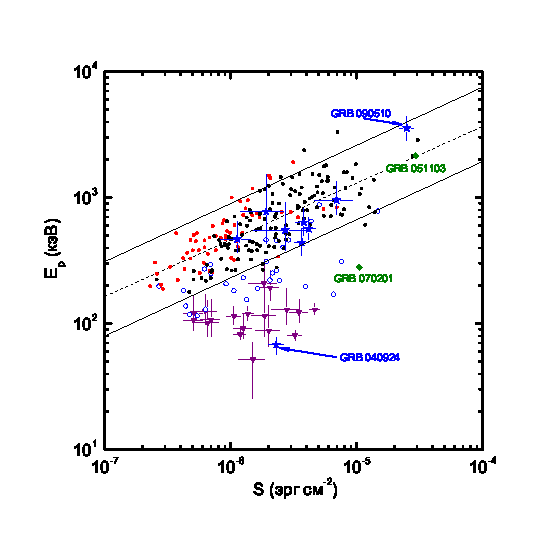
\includegraphics[width=1\textwidth]{gEpvsFl_ru.eps} \\ а)}
    \end{minipage}
    \hfill
    \begin{minipage}[h]{0.5\textwidth}
		\center{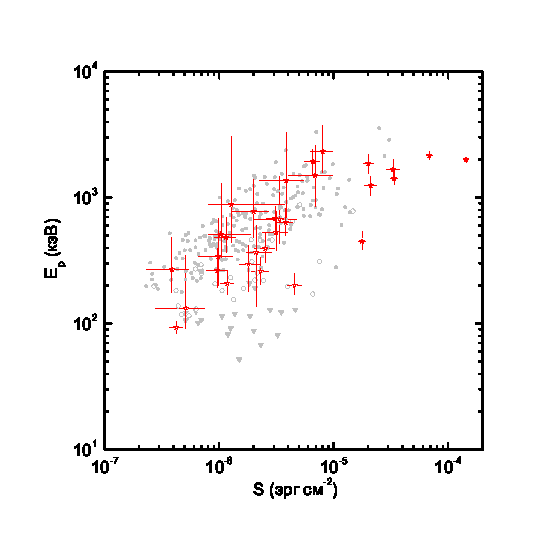
\includegraphics[width=1\textwidth]{gEpvsFlEE_ru.eps} \\ б)}
	\end{minipage}
    \vfill
    \begin{minipage}[h]{0.5\textwidth}
		\center{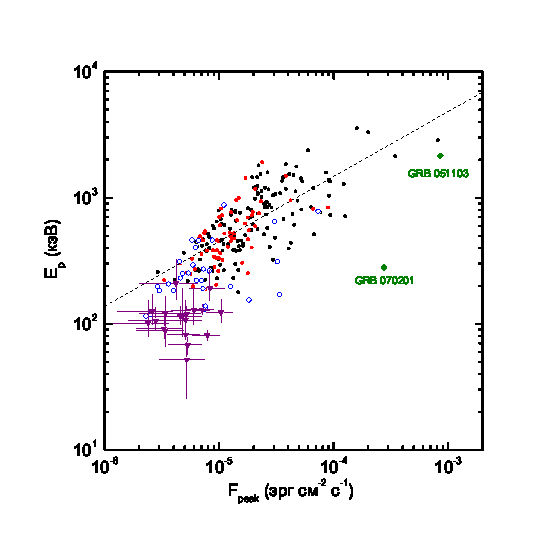
\includegraphics[width=1\textwidth]{gEpvsPF_ru.eps} \\ в)}
    \end{minipage}
    \hfill
    \begin{minipage}[h]{0.5\textwidth}
		\center{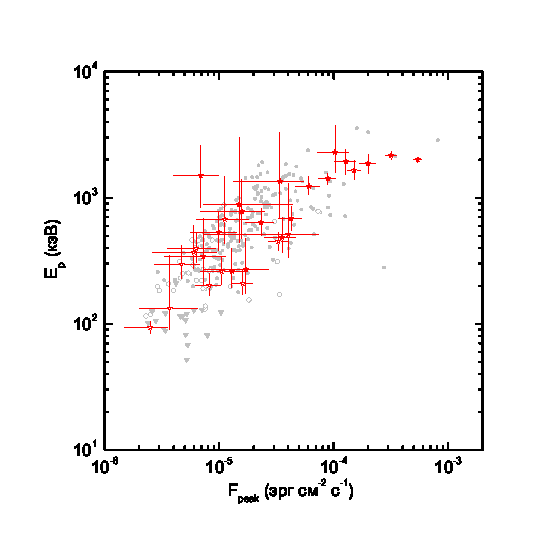
\includegraphics[width=1\textwidth]{gEpvsPFEE_ru.eps} \\ г)}
	\end{minipage}
    
\caption{\small
    Соотношение $E_\rmn{p}$ с $S$ и $F_\rmn{peak}$ для всплесков, описываемых моделью CPL.
    На панели~(а) показано соотношение $E_\rmn{p}$ и $S$ для
    всплесков типа~I с многоканальными спектрами (чёрные точки); 
    всплесков типа~I с трёхканальными спектрами (красные точки); 
    всплесков неопределённого типа (пустые точки), для обоих типов спектров;
    и для всплесков типа~II (треугольники). 
    На панели~(б) показаны всплески типов Iee (заполненные звёзды) и~Iee/II (пустые звёзды);
    остальные всплески из набора показаны серым.
    На панелях~(в) и~(г) показаны соотношение $E_\rmn{p}$ и $F_\rmn{peak}$ 
    для тех же наборов всплесков. Для всплесков типов~I и~I/II ошибки не показаны.
    Кандидаты в GF в близких галактиках обозначены ромбами. Звёздами показаны всплески с измеренным $z$.
    Пунктирная линия соответствует степенной аппроксимации соотношений для всплесков типа~I,
    в обоих случаях индекс близок к $0.5$.
    % $E_\rmn{p}$--$S$ $\lambda = 0.45 \pm 0.16$
    % $E_\rmn{p}$--$F_\rmn{peak}$ $\lambda = 0.51 \pm 0.22$
    \label{fig:EpvsFPandFL}}
\end{figure}


Интегральные распределения $\log N$--$\log S$ и $\log N$--$\log F_\rmn{peak}$
для набора 293-х коротких всплесков KW, а так же степенные распределения с индексом $-3/2$, 
соответствующие однородному распределению источников всплесков в пространстве,
представлены на рис.~\ref{fig:logNlogS_PF}.
Распределение $\log N$--$\log S$ следует однородному распределению в узкой 
области интегральных потоков $(\sim 4\textrm{--}10)\times 10^{-6}$~эрг~см$^{-2}$.
В то время как недостаток слабых всплесков может быть объяснён эффектами селекции,
наблюдаемый избыток интенсивных всплесков в значительной мере обусловлен событиями 
не относящимися к <<классическим>> коротким/жестким всплескам. Среди 12-и наиболее 
интенсивных всплесков в наборе KW с $S \gtrsim 10^{-5}$~эрг~см$^{-2}$ только 
четыре имеют Тип~I, остальные классифицированы как типы I/II, II или являются всплесками с EE.
При рассмотрении только всплесков Типа~I, соотношение $\log N$--$\log S$ хорошо 
описывается крутым показателем степени $-1.8 \pm 0.3$ выше $S\sim 5\times 10^{-6}$~эрг~см$^{-2}$.
Распределение $\log N$--$\log F_\rmn{peak}$ коротких всплесков KW также более пологое 
по сравнению с наклоном $-3/2$ и описывается показателем степени 
$-1.16 \pm 0.12$ для $F_\rmn{peak}$ лежащего в интервале
$(0.2\textrm{--}9.4)\times 10^{-4}$~эрг~см$^{-2}$~с$^{-1}$.
В том же диапазоне показатель степени для всплесков Типа~I имеет более крутой показатель 
$-1.42 \pm 0.16$, который согласуется с однородным распределением источников в пространстве.

\begin{figure}
    \begin{minipage}[h]{0.5\textwidth}
		\center{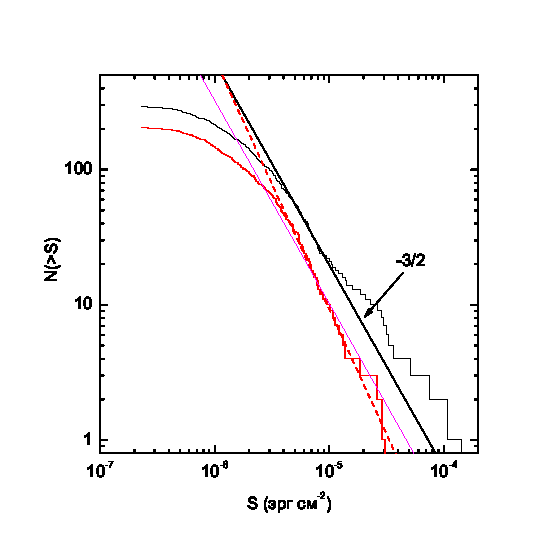
\includegraphics[width=1\textwidth]{glogNlogS_ru.eps} \\ а)}
    \end{minipage}
    \hfill
    \begin{minipage}[h]{0.5\textwidth}
		\center{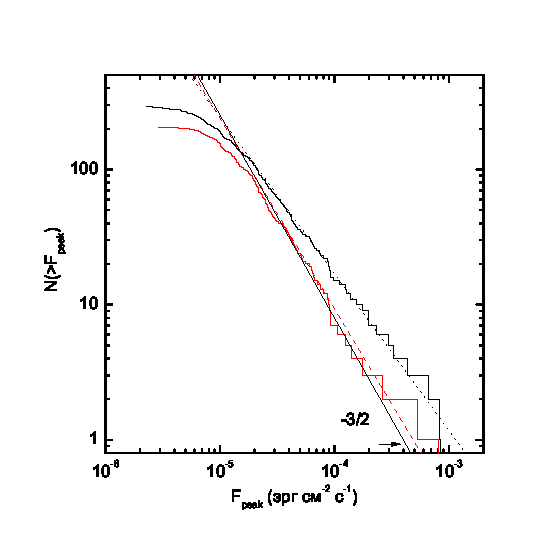
\includegraphics[width=1\textwidth]{glogNlogPF_ru.eps} \\ б)}
	\end{minipage}
\caption{
    Интегральные распределения $\log N$--$\log S$~(а) и $\log N$--$\log F_\rmn{peak}$~(б).
    Чёрные гистограммы показывают интегральные распределения для всех всплесков, 
    красные~--- только для всплесков Типа~I. Сплошные прямые линии обозначают 
    степенное распределение с показателем степени $-3/2$ и различными нормировками, 
    ожидаемое для однородного расположения источников всплесков в Евклидовом пространстве.
    Пунктирные линии показывают степенную аппроксимацию распределений всплесков Типа~I.
    На панели~(б) штриховой линией показана аппроксимация распределения всех всплесков 
    (см. параметры и диапазоны аппроксимаций в тексте).
    \label{fig:logNlogS_PF} }
\end{figure}

Иллюстрации временных историй и спектров 214 коротких всплесков KW, а также таблицы размещены на сайте
ФТИ~им.~А.Ф.~Иоффе\footnote{http://www.ioffe.ru/LEA/shortGRBs/Catalog2/}.

\section{Заключение}
В данной главе представлен спектральный анализ коротких гамма-всплесков Конус-Винд.
По материалам Главы~\ref{sGRB_spectral_catalog} на защиту выносится следующие положения:
\begin{enumerate}
\item Каталог с результатами спектрального анализа коротких гамма-всплесков, 
    зарегистрированных в эксперименте Конус-Винд.
\item Обнаружение дополнительной спектральной компоненты у коротких гамма-всплесков, 
    зарегистрированных в эксперименте Конус-Винд.
\item Результаты поиска, временные и спектральные характеристики коротких гамма-всплесков 
    с продленным излучением, зарегистрированных в эксперименте Конус-Винд.
\end{enumerate}

Результаты отражены в публикации\\
D.~S.~Svinkin, D.~D.~Frederiks, R.~L.~Aptekar, et al. 
The second Konus-\textit{Wind} catalog of short gamma-ray bursts //
submitted to ApJS

Автор лично произвел спектральный анализ описанного набора коротких гамма-всплесков.
Интерпретация результатов была сделана совместно с соавторами при активном участии автора.

\clearpage